\section{Results}
\label{sec:results}

%The data-driven probabilistic model we have presented can be applied in many different ways to produce diverse coloring suggestions. The factor graph representation can easily adapt to new scenarios or incorporate user-provided design constraints by introducing additional factors to the factor graph, or by changing the source data used to train the factor weights and color property distributions.

In this section, we demonstrate the flexibility of our model when applied to a variety of pattern coloring scenarios. Results were generated using a model trained on patterns from the 10 most popular artists in our dataset, except for patterns with a template used in a result figure or experiment; the training patterns and final weights for each of our factors can be found in the supplemental materials. To sample from the model, we used parallel tempering with 5 chains at temperatures $(1, 0.5, 0.2, 0.05, 0.01)$, swapping colors between chains every 50 iterations. We then used MMR to retrieve a diverse set of samples from the resulting MCMC chains. Images were rendered using the COLOURlovers online pattern creator, from color assignments generated by our model.

\subsection{Coloring Pattern Templates}

People can color patterns with a variety of different criteria in mind, which may even change during the coloring process. These preferences can range from the more general preference for any appealing coloring to more specific preferences such as using a particular palette, looking for local improvements to an existing coloring, or matching a specific style. We explore how our model can facilitate these scenarios.

%People can color patterns with a variety of different criteria in mind. Some have no specific preferences and are looking for any well-colored pattern. Others might have a specific color palette in mind and are looking for patterns that use exactly this palette. Still others might have a general idea of the coloring they want but would like to see if it can be improved upon. Finally, some people might want colorings that conform to a particular style, such as the style of a specific artist, or a more general style such as ``bright'' or ``dark''. Below, we explore how our model can help with each of these scenarios.

\paragraph{Automatic pattern coloring} In the most direct application of our framework, we can sample from our model to produce colorings for a pattern template that are similar to the colorings used for training. Figure~\ref{fig:teaser} shows two examples of this process. The sampled patterns exhibit a range of colors and styles employed by the COLOURLovers artists. For comparison, the same patterns colored with palettes randomly sampled from RGB-space are shown on the right. These patterns exhibit significant problems, such as low color harmony and adjacent regions with equi-luminant colors.

\paragraph{Coloring with fixed palettes} 

Artists often draw inspiration from inspirational photographs and existing color themes, and may have specific colors in mind when coloring in a pattern. However, even with a fixed palette of colors, there are still a range of images that can be created by mapping different colors to different regions, some more desirable than others. To support this scenario, we use our model's score to rank all possible permutations of the colors, excluding the O'Donovan color compatibility factor.

Figure~\ref{fig:photographMatching} shows an example where colors from two photographs are applied to different pattern templates. A color palette is first automatically extracted from the input photograph~\cite{SharonPaletteExtraction}. Our algorithm then automatically computes a pleasing mapping from the colors in the extracted palette to regions in a given pattern template.~\remark{Comment on e.g. why does it use white for the background?} 

\begin{figure}[h!]
\begin{tabular}{cccc} 
\raisebox{0.5em}{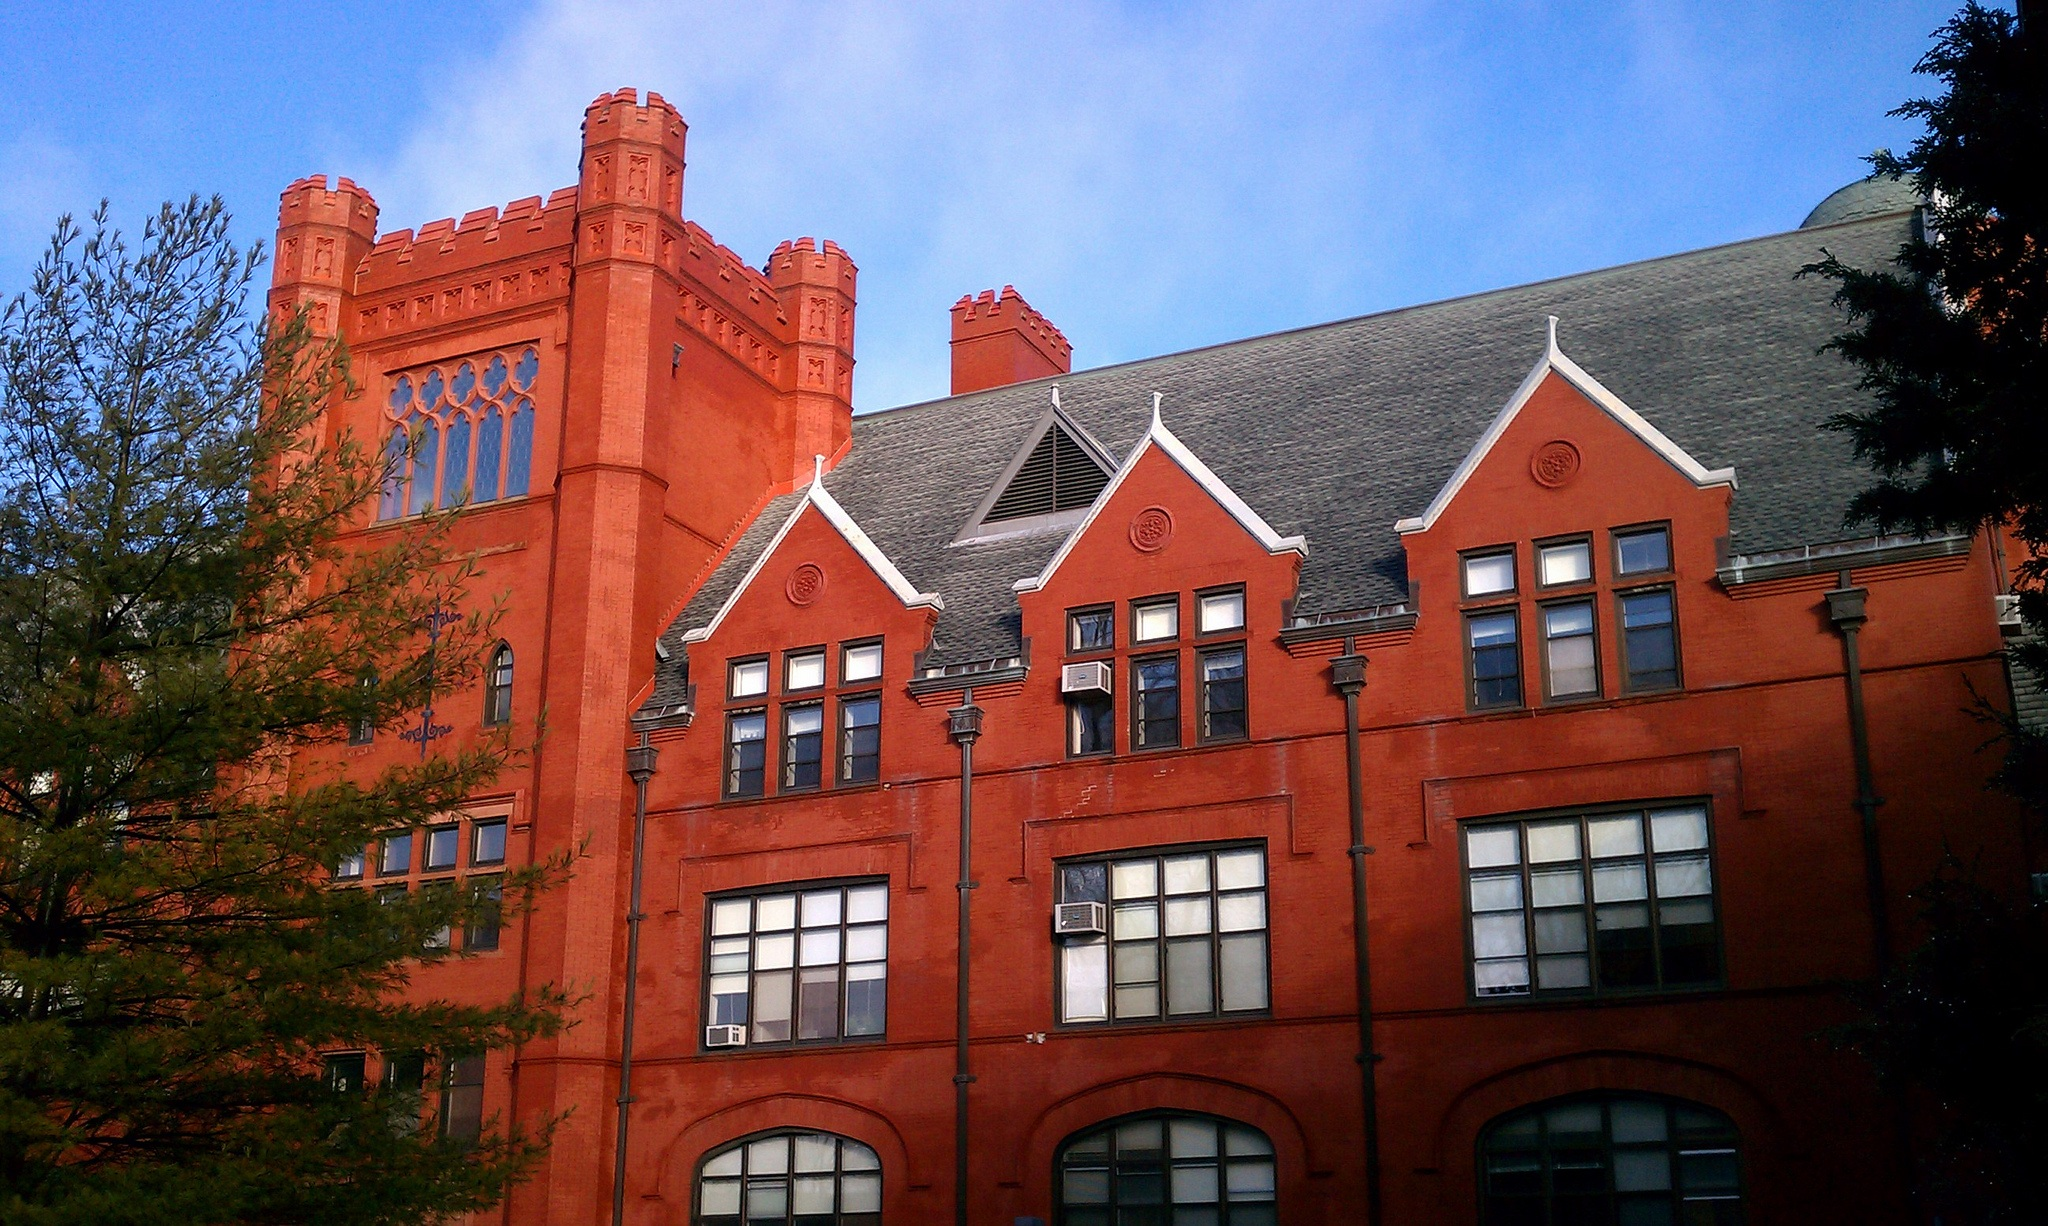
\includegraphics[width=.275\columnwidth]{figs/photos/brick}}&
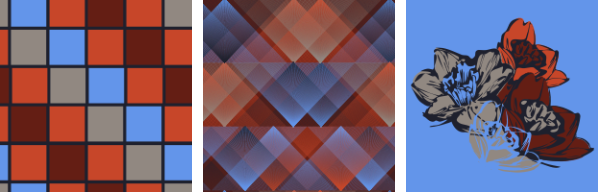
\includegraphics[width=.65\columnwidth]{figs/photos/brickAll}\\
\raisebox{0.5em}{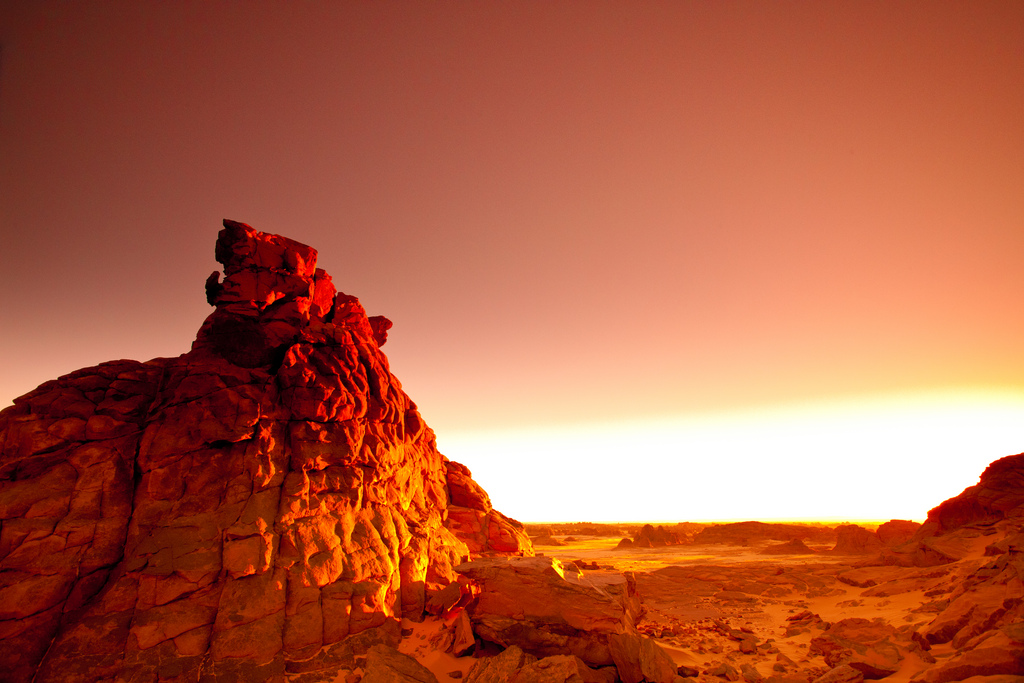
\includegraphics[width=.275\columnwidth]{figs/photos/sunset}}&
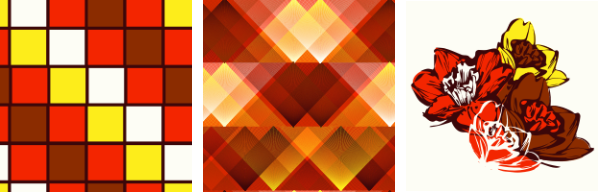
\includegraphics[width=.65\columnwidth]{figs/photos/sunsetAll}
\end{tabular}

\caption{Palettes are extracted from the two input photographs on the left, and on the right we show the top-scoring coloring suggested by our algorithm for three different pattern templates.}
\vspace{-1.0em}
\label{fig:photographMatching}
\end{figure}


\begin{figure*}[ht!]
\begin{tabular}{ccc}
\raisebox{1.2em}{
\includegraphics[width=.15\linewidth]{figs/permutationTemplateBird}} & 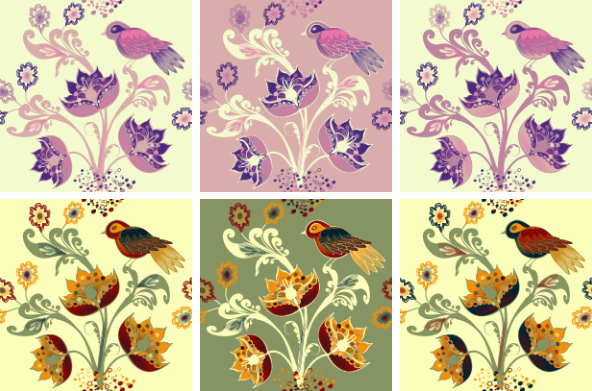
\includegraphics[width=.39\linewidth]{figs/permutationBest3} & 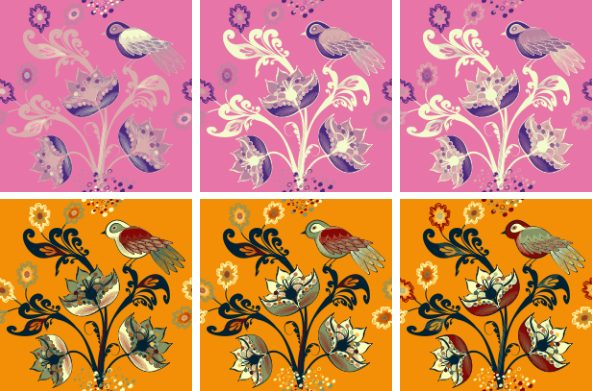
\includegraphics[width=.39\linewidth]{figs/permutationWorst3} %& 
\includegraphics[width=.12\linewidth]{figs/permutationArtist}
  \\
\textbf{(a)} Input Palettes & \textbf{(b)} Highest-scoring assignments & \textbf{(c)} Lowest-scoring assignments %& \textbf{(d)} Artist assignment
\\
\end{tabular}

\caption{Given a pattern template and corresponding palette as input, we use our color model to compute the score of each possible assignment of the palette to the image regions. \textbf{(b)} and \textbf{(c)} show the top-3 and bottom-3 assignments for two different palettes.}
\label{fig:permutation}
\end{figure*}

\begin{figure*}[ht]
\begin{tabular}{cc} 
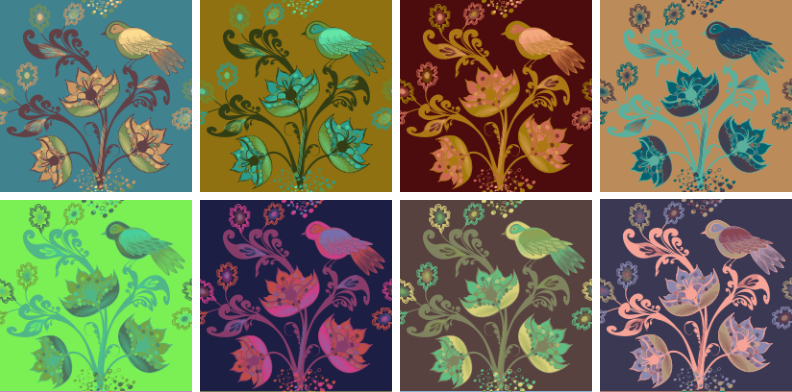
\includegraphics[width=.475\linewidth]{figs/constrainedSearchUnconstrained}&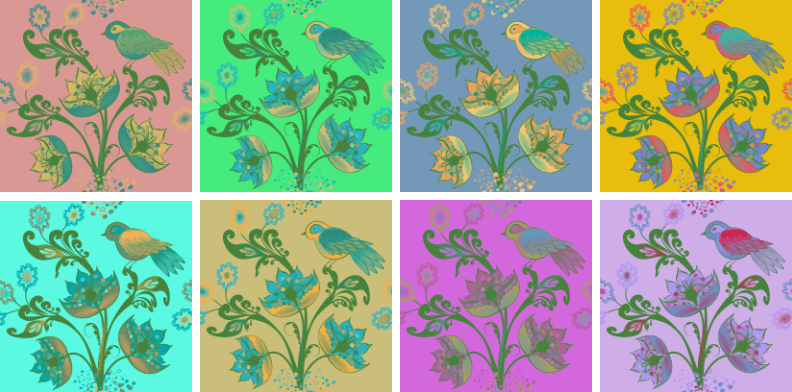
\includegraphics[width=.475\linewidth]{figs/constrainedSearchConstrained}\\
Initial automatic suggestions & After fixing the stem to be green\\
\end{tabular}

\caption{An artist coloring a pattern is presented with the results shown on the left, and decides that she only likes results where the stem of the plant is dark green. On the right, we use conditional inference to sample from our model subject to the constraint that the desired palette entry is fixed to a specific color.}
\label{fig:constrainedInference}
\vspace{-1.0em}
\end{figure*}


Although using a pleasing palette often improves the look of a pattern, the spatial arrangement of those colors can make a dramatic difference in appearance. Figure~\ref{fig:permutation}, shows two input color palettes for the bird pattern and the highest and lowest-scoring color assignments to the pattern from our model. These palettes were originally created by artists beforehand either from scratch or from a photograph, and were actually applied to this pattern on COLOURlovers. Our model ranks the original artist-created color assignments as 39st (top palette) and 21st (bottom palette) out of 120 possible permutations. This suggests that the model may be capturing general artist trends in pattern coloring.

In this example, the model terms that most distinguish the 3 highest-scoring assignments from the 3 lowest-scoring assignments are the group and segment color name counts. Our model prefers colors like yellow, grey, and green to red-orange and orange-brown for background colors. Assignments with these orange background colors tend to be ranked the lowest. This may be because there are few popular patterns with orange backgrounds in our training set.


\paragraph{Hard color constraints}

In some cases, a user may only have partial knowledge about the colors she wants to see in particular pattern regions. Our model can assist users in this situation by fixing the color of certain pattern regions and using conditional inference to sample values for the remaining unconstrained color variables. Figure~\ref{fig:constrainedInference} shows an example, where after viewing the initial suggestions, the user decides she wants to see more results where the stem of the plant is a particular green, and our system outputs new suggestions subject to this constraint.~\remark{Comment on the effect this has (i.e. it makes other regions more likely to also be green, etc.)}

\paragraph{Soft color constraints}

In another use case, a user might have strong preferences for the appearance of the pattern. She might manually color a pattern and then wish to see variations upon this theme, hoping to find better-looking alternatives nearby in the space of colorings. Our model can support this type of query by incorporating an additional soft constraint factor on color variable, constraining it ot be close to a target color:
%%
\begin{equation}
\factor^\textrm{Target}(\colorVars_\group | \pattern) = \mathcal{N}(||\colorVars_\group - \textrm{targetColor}(\group)||, \sigma_\textrm{user})
\label{eq:targetFactor}
\end{equation}
%%
Here, $\textrm{targetColor}(\group)$ is the desired color of group $\group$ and $\sigma_\textrm{user}$ controls the extent to which the group is allowed to deviate from the desired color. We assign this factor a weight $w_\textrm{user} * w_\textrm{model}$, where $w_\textrm{model}$ is the sum of the weights of all other factors in the model. $w_\textrm{user}$ controls the tradeoff between satisfying the user-specified target colors for a region versus satisfying the color distribution encoded by the trained model.
%
%This factor corresponds to adding a new term in our log-linear model with this statistics function:
%%%
%\begin{equation*}
%\termStats(\colors | \pattern) = \sum_{\group \in \groups}{\ln \mathcal{N}(||\colors_\group - \textrm{targetColor}(\group)||, \sigma_\textrm{user})}
%\end{equation*}
%%%

%\begin{figure}[ht]
%\begin{tabular}{cc}
%{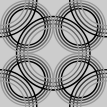
\includegraphics[width=.1785\columnwidth]{figs/brightness0Original}}&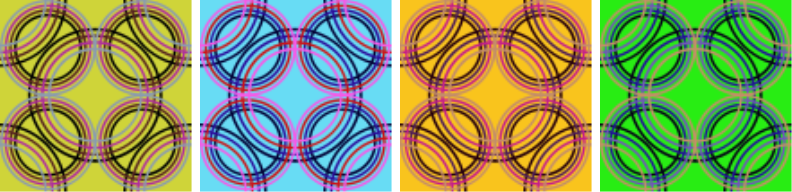
\includegraphics[width=.735\columnwidth]{figs/brightness0MMR}\vspace{0.5em}\\
%{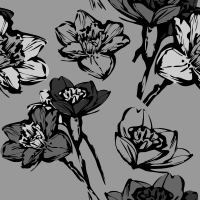
\includegraphics[width=.1785\columnwidth]{figs/brightness1Original}}&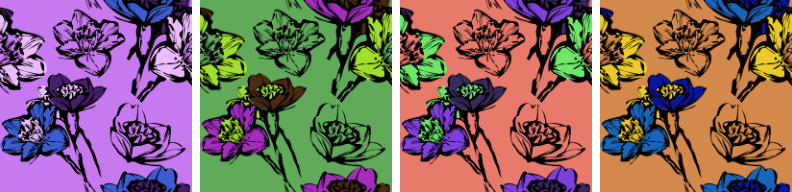
\includegraphics[width=.735\columnwidth]{figs/brightness1MMR}\vspace{0.5em}\\
%\raisebox{2em}{
\includegraphics[width=.22\columnwidth]{figs/guidedSearch2Original}}%&
\includegraphics[width=.7\columnwidth]{figs/guidedSearch2MMR}\\
%Original&Suggestions\\
%\end{tabular}

%\caption{TODO.}
%\label{fig:lightnessSearch}
%\vspace{-1.0em}
%\end{figure}

\begin{figure}[!h]
\begin{tabular}{cc}
{
\includegraphics[width=.1785\columnwidth]{figs/guidedSearch1Original}}&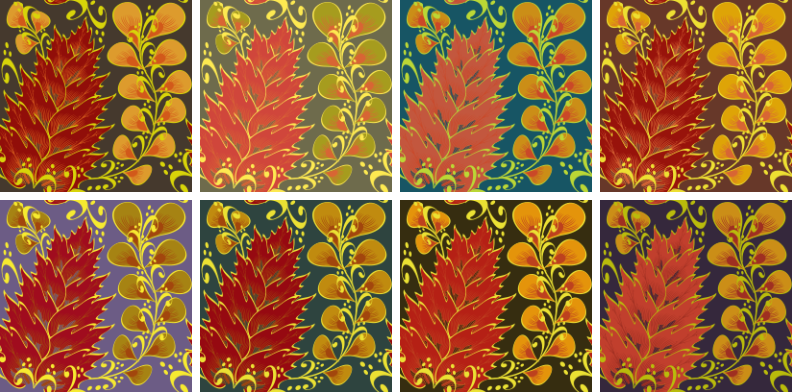
\includegraphics[width=.735\columnwidth]{figs/guidedSearch1MMR}\vspace{0.5em}\\
{
\includegraphics[width=.1785\columnwidth]{figs/guidedSearch0Original}}&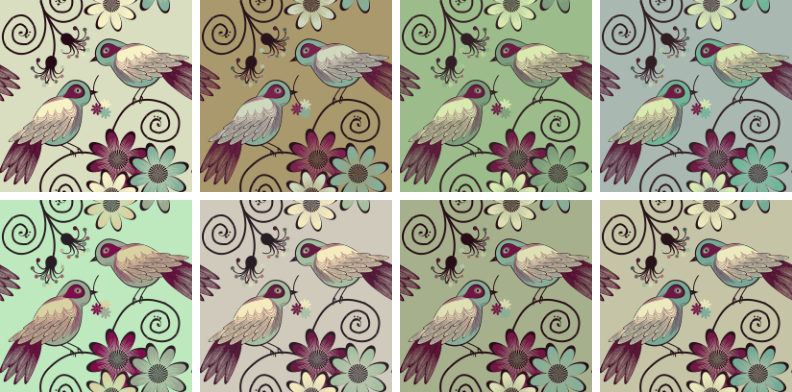
\includegraphics[width=.735\columnwidth]{figs/guidedSearch0MMR}\vspace{0.5em}\\
%\raisebox{2em}{
\includegraphics[width=.22\columnwidth]{figs/guidedSearch2Original}}%&
\includegraphics[width=.7\columnwidth]{figs/guidedSearch2MMR}\\
Original&Suggestions\\
\end{tabular}

\caption{An artist provides an initial color assignment and asks for patterns that are similar. We incorporate this request by adding an additional factor to our model, showing four samples drawn from the new model for each of the input images.}
\label{fig:nearbySuggestions}
\vspace{-1.0em}
\end{figure}

Figure~\ref{fig:nearbySuggestions} shows example scenarios where a proposed coloring is given, and the model returns similar colorings. Here we choose $\sigma_\textrm{user}$ to be 10\% of the diagonal length of the \lab color space, and $w_\textrm{user}=3$, indicating a desire to remain fairly close to the original coloring. Our model is able to make numerous variations to the input colors while still preserving the overall quality of the results.

\begin{figure}[ht]
\begin{tabular}{ccc} 
Style&Example&Results\\ %\hline
\raisebox{1.55em}{\emph{Light}}&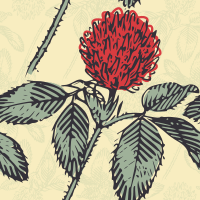
\includegraphics[width=.148\columnwidth]{figs/styleResultsLightExample}&
\includegraphics[width=.62\columnwidth]{figs/styleResultsLight}\vspace{0.5em}\\
\raisebox{1.55em}{\emph{Dark}}&
\includegraphics[width=.148\columnwidth]{figs/styleResultsDarkExample}&
\includegraphics[width=.62\columnwidth]{figs/styleResultsDark}\vspace{0.5em}\\
\raisebox{1.55em}{\emph{Bold}}&
\includegraphics[width=.148\columnwidth]{figs/styleResultsBoldExample}&
\includegraphics[width=.62\columnwidth]{figs/styleResultsBold}\vspace{0.5em}\\
\raisebox{1.55em}{\emph{Mellow}}&
\includegraphics[width=.148\columnwidth]{figs/styleResultsMellowExample}&
\includegraphics[width=.62\columnwidth]{figs/styleResultsMellow}\vspace{0.5em}\\
\end{tabular}

\caption{In this example, 17 patterns were chosen in three different styles, and a representative image from each style is shown in the second column. A separate model was then trained on each style, and in the third column we show four samples drawn from each model. In each case, our model is able to learn different properties of the desired distribution over colors.}
\label{fig:styleTraining}
\vspace{-1.0em}
\end{figure}

\begin{figure*}[ht]
\begin{tabular}{cc} 
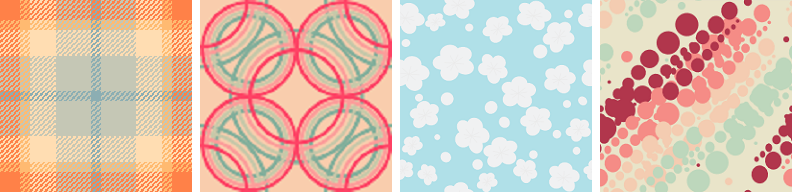
\includegraphics[width=.48\linewidth]{figs/styleSugarExamples}&
\includegraphics[width=.48\linewidth]{figs/styleAlbenajExamples}\vspace{1.0em}\\
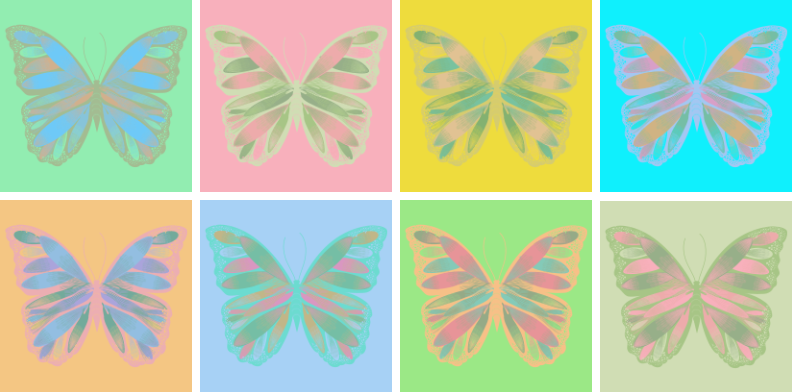
\includegraphics[width=.48\linewidth]{figs/styleSugar}&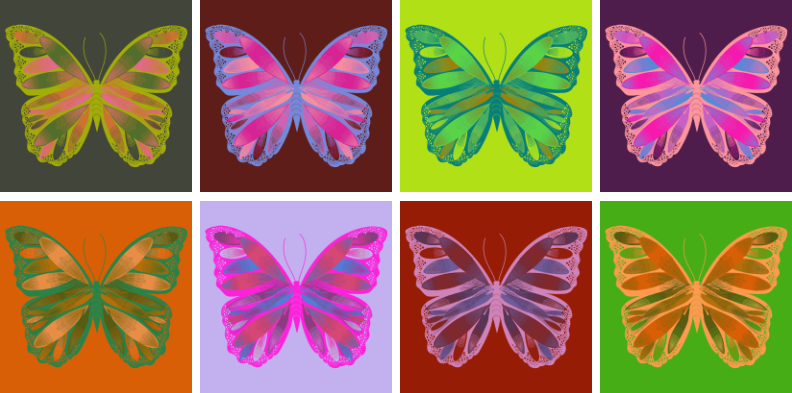
\includegraphics[width=.48\linewidth]{figs/styleAlbenaj}\\
Artist A&Artist B\\
\end{tabular}

\caption{Our data-driven approach makes it easy to capture the styles of different artists. Top: representative images from two different artists. Bottom: results sampled from a model trained on 100 images from the artist.}
\vspace{-1.0em}
\label{fig:artistTraining}
\end{figure*}

\paragraph{Style capture} A powerful advantage of a data-driven approach is the ability to modify the underlying training source to achieve specialization of the resulting model. This ability allows our model to capture a specific style and color preferences such as ``high-contrast patterns'' by selecting a set of patterns with the desired property. Figure~\ref{fig:styleTraining} demonstrates this behavior using four style categories: \emph{Light}, \emph{Dark}, \emph{Bold}, and \emph{Mellow}. Using 17 training examples, our model can capture general properties of the example patterns such as the distribution of colors over the background regions in \emph{Light} and \emph{Dark} and the amount of contrast between regions in \emph{Bold} and \emph{Mellow}. The model can also capture the style of a specific artist, as shown in Figure~\ref{fig:artistTraining}. Here, 100 images from each artist were used for training. The sampled images mimic certain properties of the the style of each artist, such as the light backgrounds preferred by artist A and the bold colors and dark backgrounds preferred by artist B. The complete list of patterns used as training data for these examples can be found in the supplemental materials.

\subsection{Applications}

Next, we show how our model can be applied to real-world pattern coloring tasks, such as coloring in webpage backgrounds, coordinating colors in interior scene design, and suggesting clothing colorings to fit people with different physical attributes. %We show how to color the background of a webpage to match different foreground color themes, how to improve the color coordination of interior scene designs, and how to suggest colorings for clothing patterns to fit people with different physical attributes.

\paragraph{Web design}
A web designer may want to change a web page's color theme to fit the season, a special event, or even the time of day. Our model can support this tasks by suggesting recolorings for web page pattern elements. In Figure~\ref{fig:webpageRecoloring}, the background pattern of a blog is automatically recolored in three distinct styles. Each style is defined by a manually-specified page body color and header text color. We generate these recolorings by adding new factors to the model. First, we add a unary factor to each color variable that encourages similarity to a color that occurs in the web page body:
%%
\begin{equation*}
\factor^\textrm{WebSim}(\colorVars_\group | \webpage) = p(\colorVars_\group | \webpage)
\end{equation*}
%%
where $\webpage$ is a rendered image of the web page body. The distribution $p$ is represented with a smoothed histogram of colors in the image, after quantizing to a small number of colors (20, in this experiment).
We also add a factor to the pattern's background color group that penalizes similarity to the web page body background color:
%%
\begin{equation*}
\factor^\textrm{BgPen}(\colorVars_{\textrm{largest}(\groups)} | \webpage) = 0.05 \cdot || \colorVars_{\textrm{largest}(\groups)} - \textrm{bgColor}(\webpage) ||
\end{equation*}
%%
This term ensures that the body of the page stands out from the rest of the page. A more sophisticated approach would treat the entire web page as a pattern and perform joint recoloring; we leave this extension to future work.


\begin{figure}[ht]
\centering

\includegraphics[width=\columnwidth]{figs/webpageRecoloring}
\caption{With a few additional factors, our model can recolor the background pattern of a web page to match the colors in the page body.}
\label{fig:webpageRecoloring}
\end{figure}

\paragraph{3D scene design}
Color-coordinating a virtual scene is another creative task that can benefit from computatational support. While repositories such as the 3D Warehouse provide a wealth of object models with which to build scenes, such models are rarely color coordinated with one another. Figure~\ref{fig:sceneRecoloring} shows how our model can make coordinating object colors easier. We can treat a scene as a recolorable pattern by rendering its material coefficients to an image. The user then provides a few additional annotations to specify which object components should be the same color; in this example, cushions, pillows, and wooden objects must take the same color. Finally, we add a factor to our model to enforce that the colors assigned to each component are similar to their original colors (see Equation~\ref{eq:targetFactor}) to keep the system from wandering into physically implausible colorings. The resulting model suggests plausible, improved recolorings of the scene.
%Our model's applicability to this task, despite it being trained only on \emph{2D} patterns, suggests that it captures some simple cross-domain aesthetic principles.

\begin{figure*}[ht]
\begin{tabular}{c|ccc} 
Original&Recoloring 1&Recoloring 2&Recoloring 3\vspace{0.4em}\\
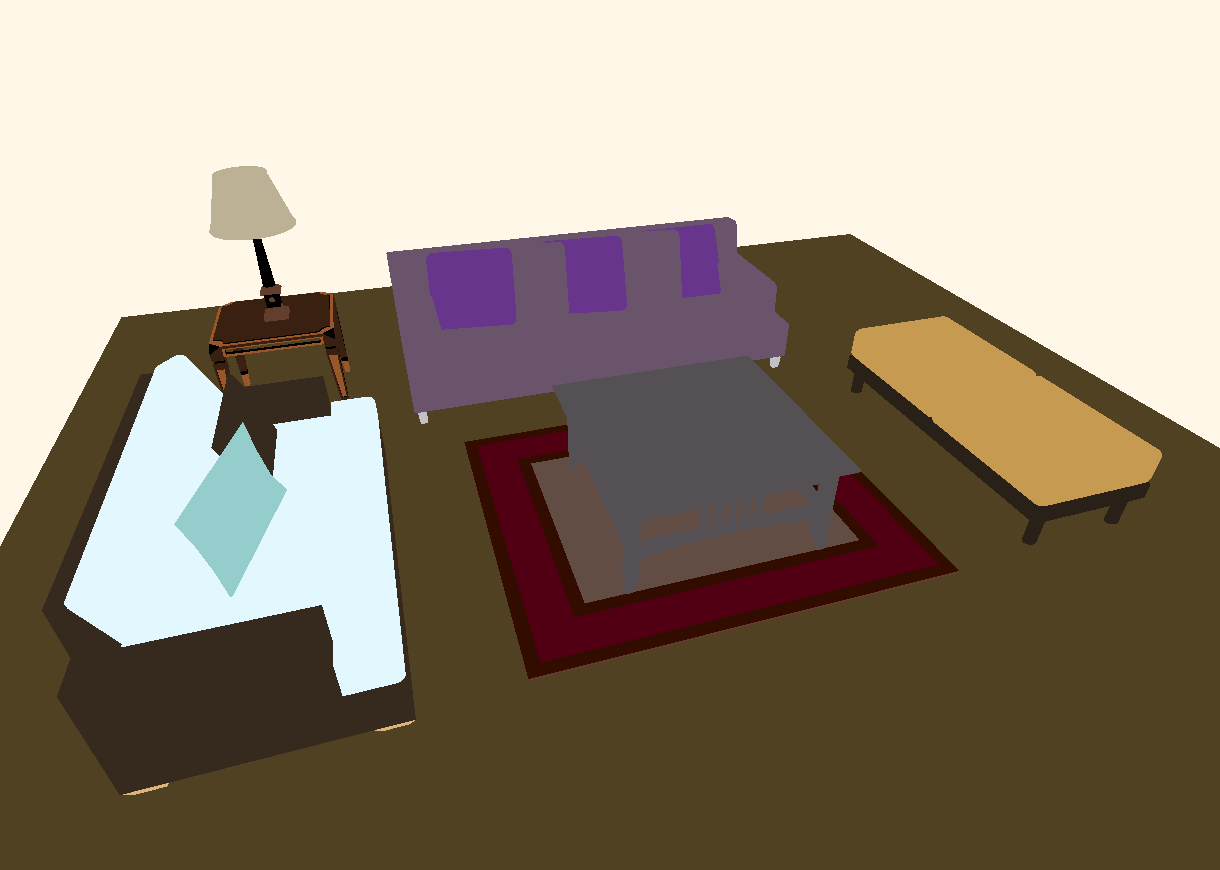
\includegraphics[width=.23\linewidth]{figs/3dscene/original}&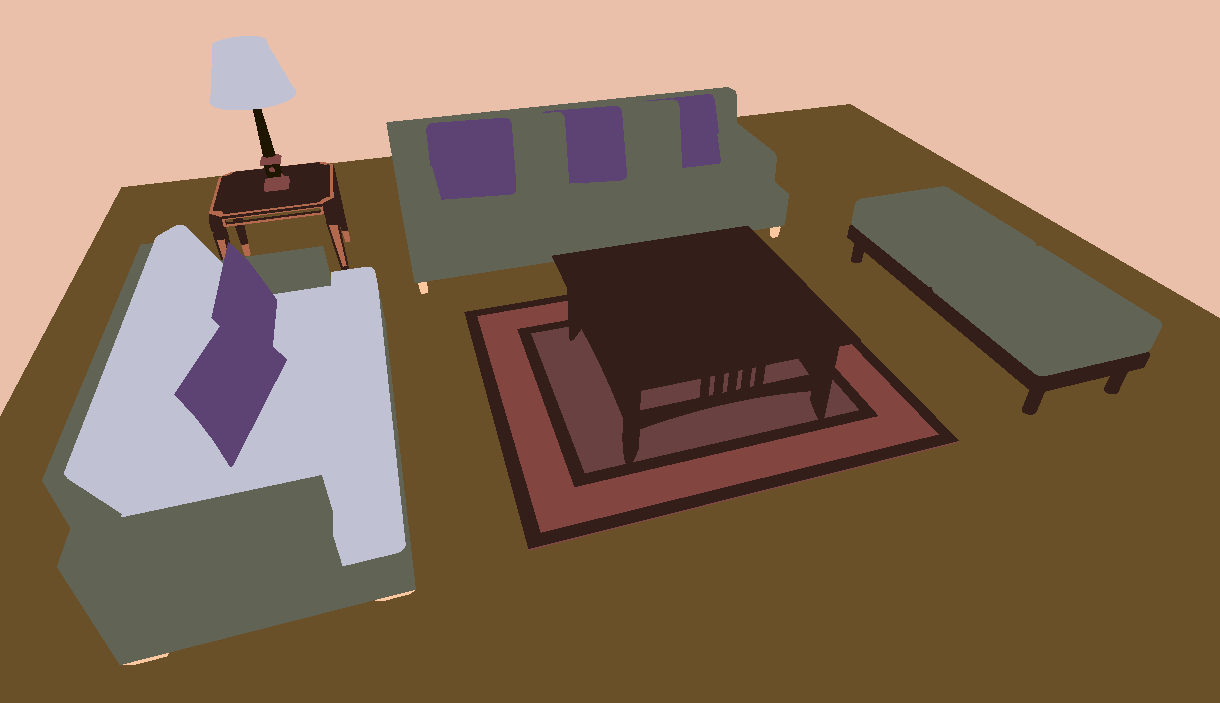
\includegraphics[width=.23\linewidth]{figs/3dscene/recolored_17}&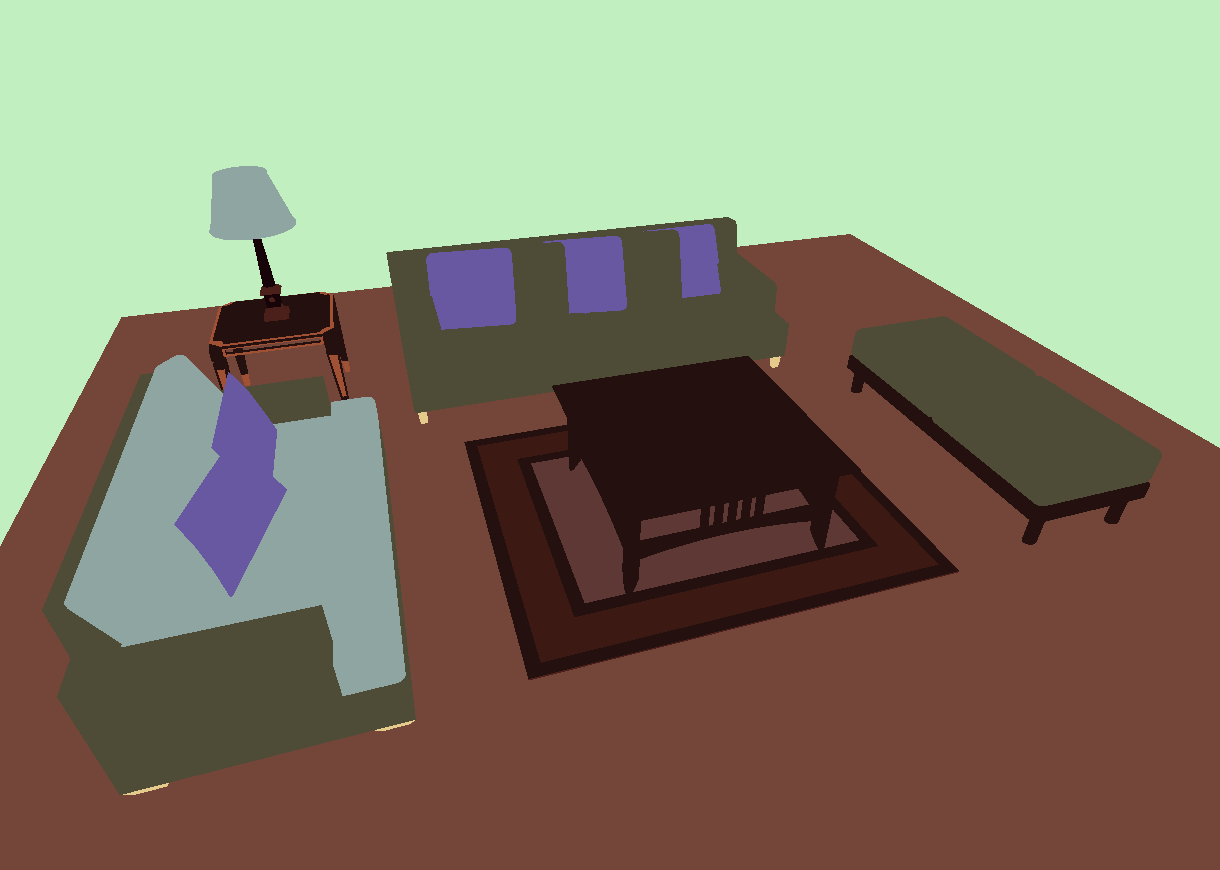
\includegraphics[width=.23\linewidth]{figs/3dscene/recolored_03}&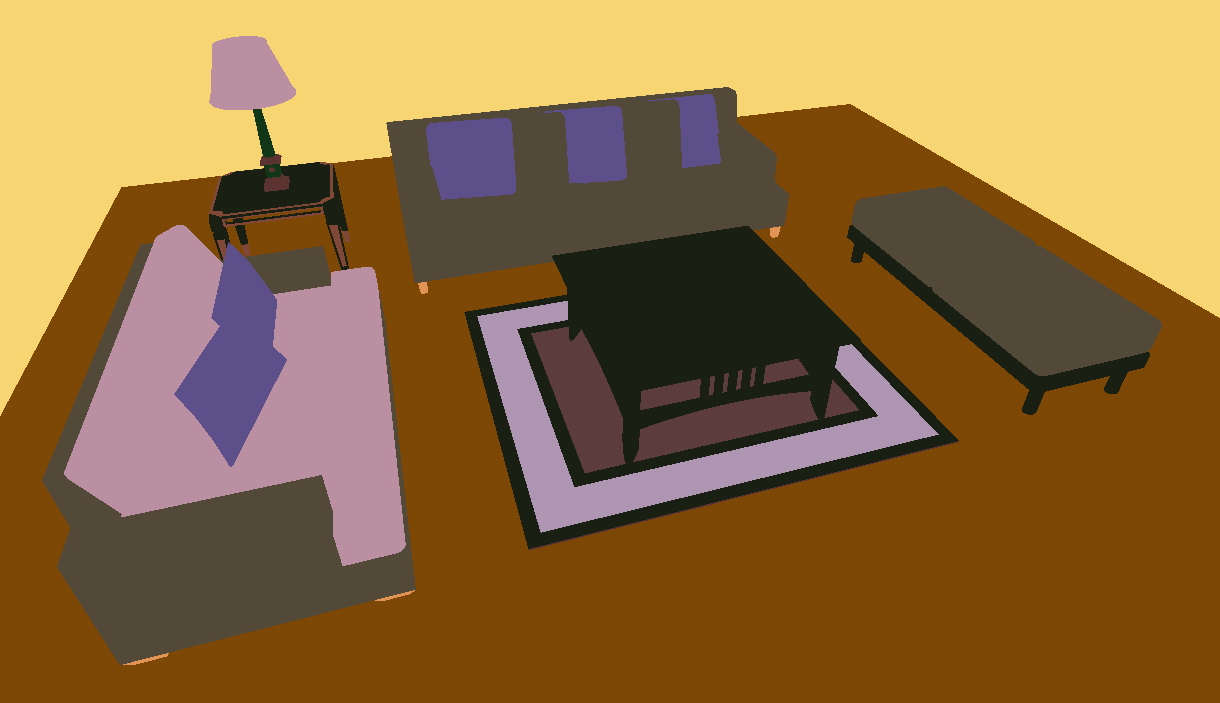
\includegraphics[width=.23\linewidth]{figs/3dscene/recolored_15}\vspace{0.4em}\\
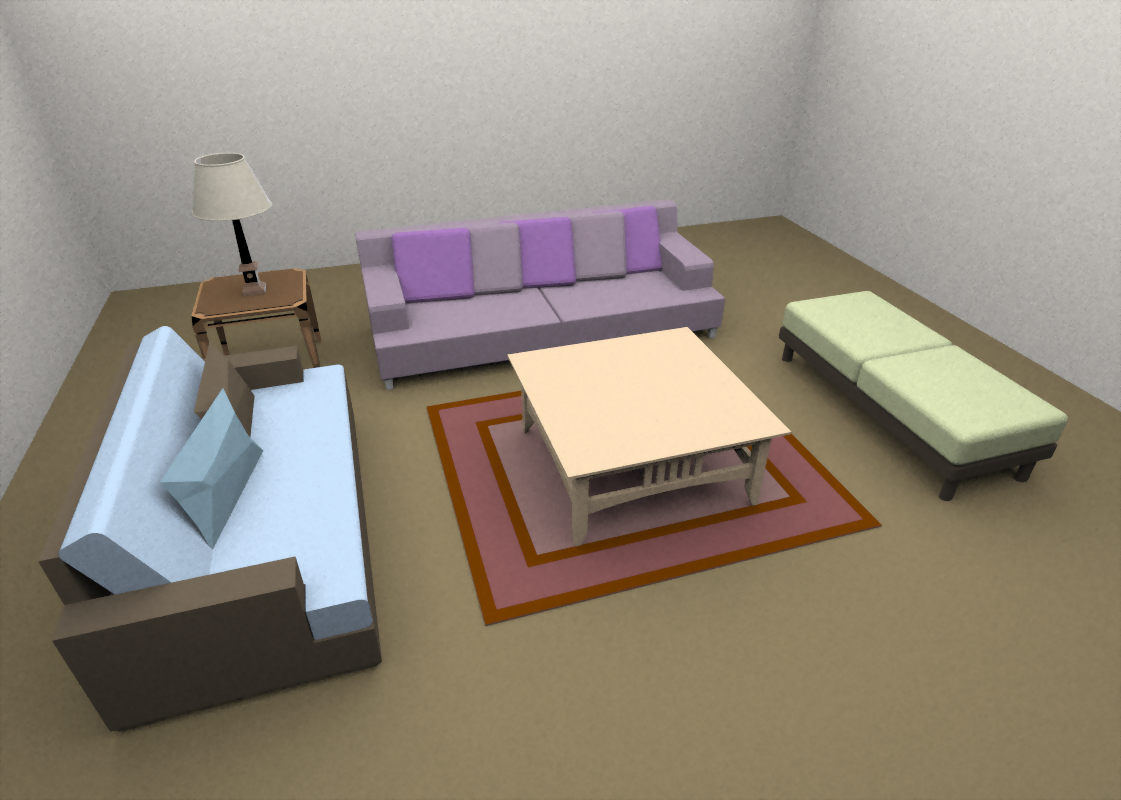
\includegraphics[width=.23\linewidth]{figs/3dscene/original_pbrt}&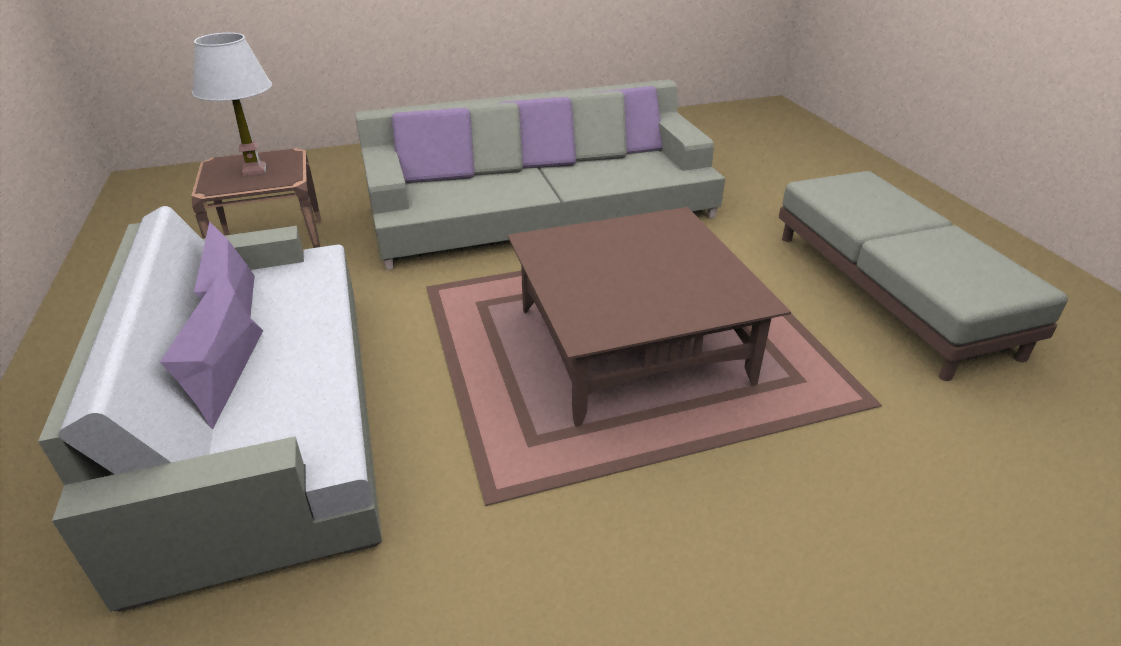
\includegraphics[width=.23\linewidth]{figs/3dscene/recolored_17_pbrt}&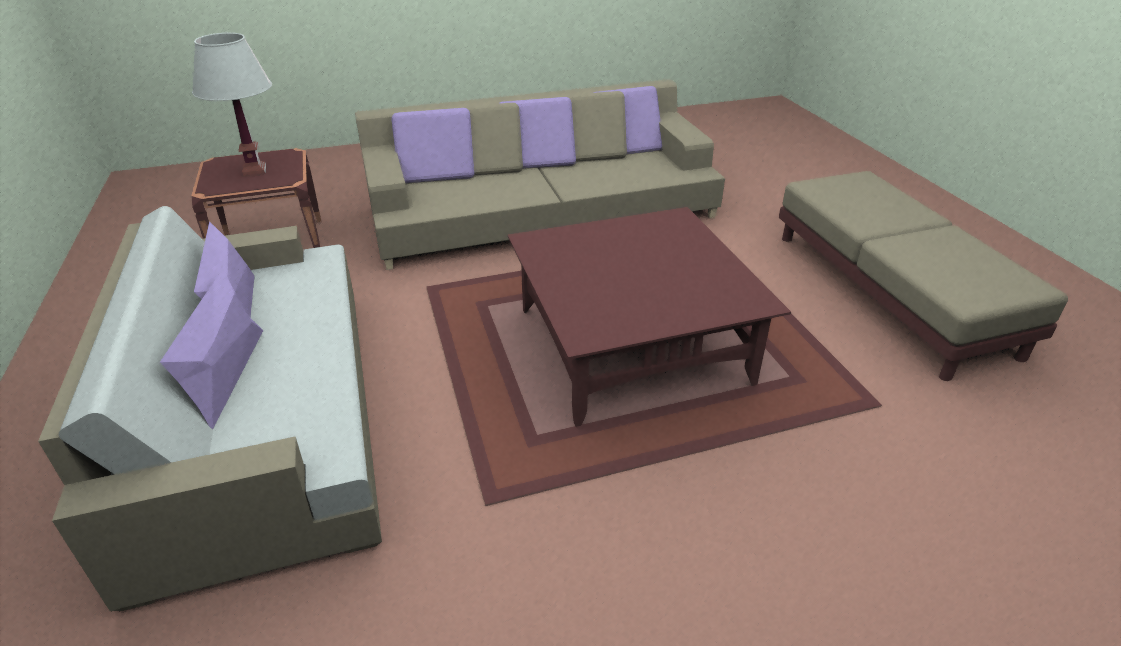
\includegraphics[width=.23\linewidth]{figs/3dscene/recolored_03_pbrt}&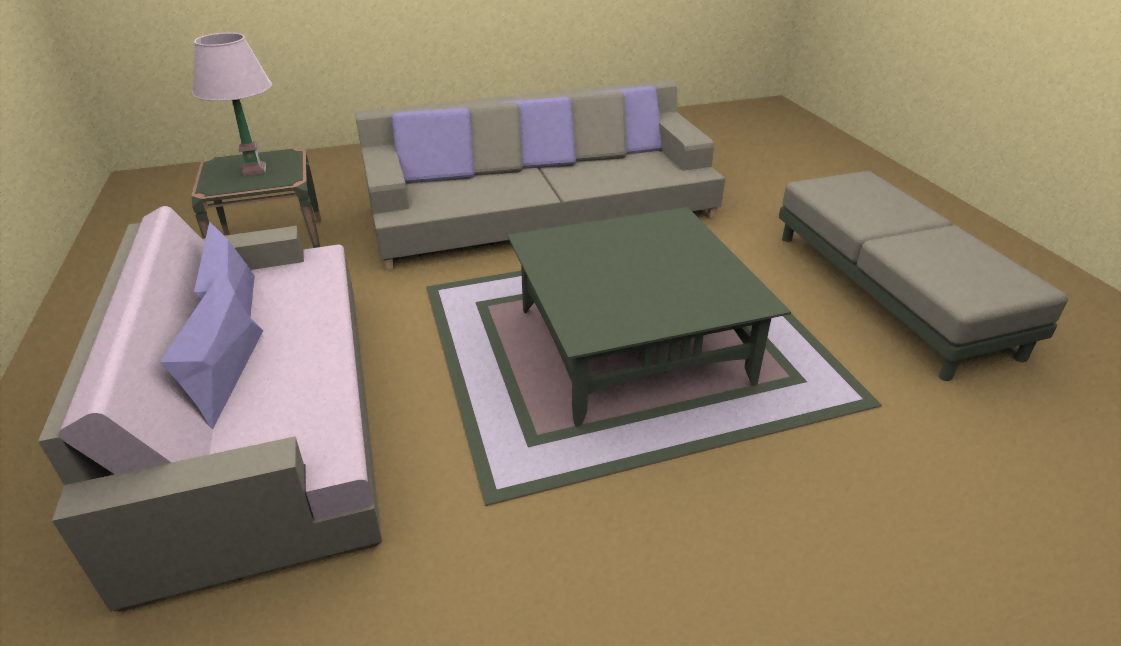
\includegraphics[width=.23\linewidth]{figs/3dscene/recolored_15_pbrt}\vspace{0.4em}\\
\end{tabular}

\caption{A poorly color-coordinated 3D scene is recolored using our model. Using the original coloring as a soft constraint, our model suggests multiple novel recolorings. (Top) Diffuse material coefficients for each object. (Bottom) Final renderings.}
\label{fig:sceneRecoloring}
\vspace{-1.0em}
\end{figure*}

\paragraph{Fashion design}
Our model can also adapt the colorings of clothing items to fit different people. Figure~\ref{fig:fashion} shows a shirt recolored to match different hair, eye, and skin tones. The hair, skin, eyes, and lips of the 3D person model were manually quantized to a single color; the resulting texture atlas functions as a recolorable pattern template. Fixing the colors of the hair, skin, eyes, and lips constrains the inference process to produce suitable colorings for a person with those physical attributes.
%It should be possible to apply a similar procedure to photographic images, though those inputs may require an intrinsic image decomposition to separate shading from reflectance~\cite{IntrinsicImages}.

\begin{figure}[ht!]
\centering
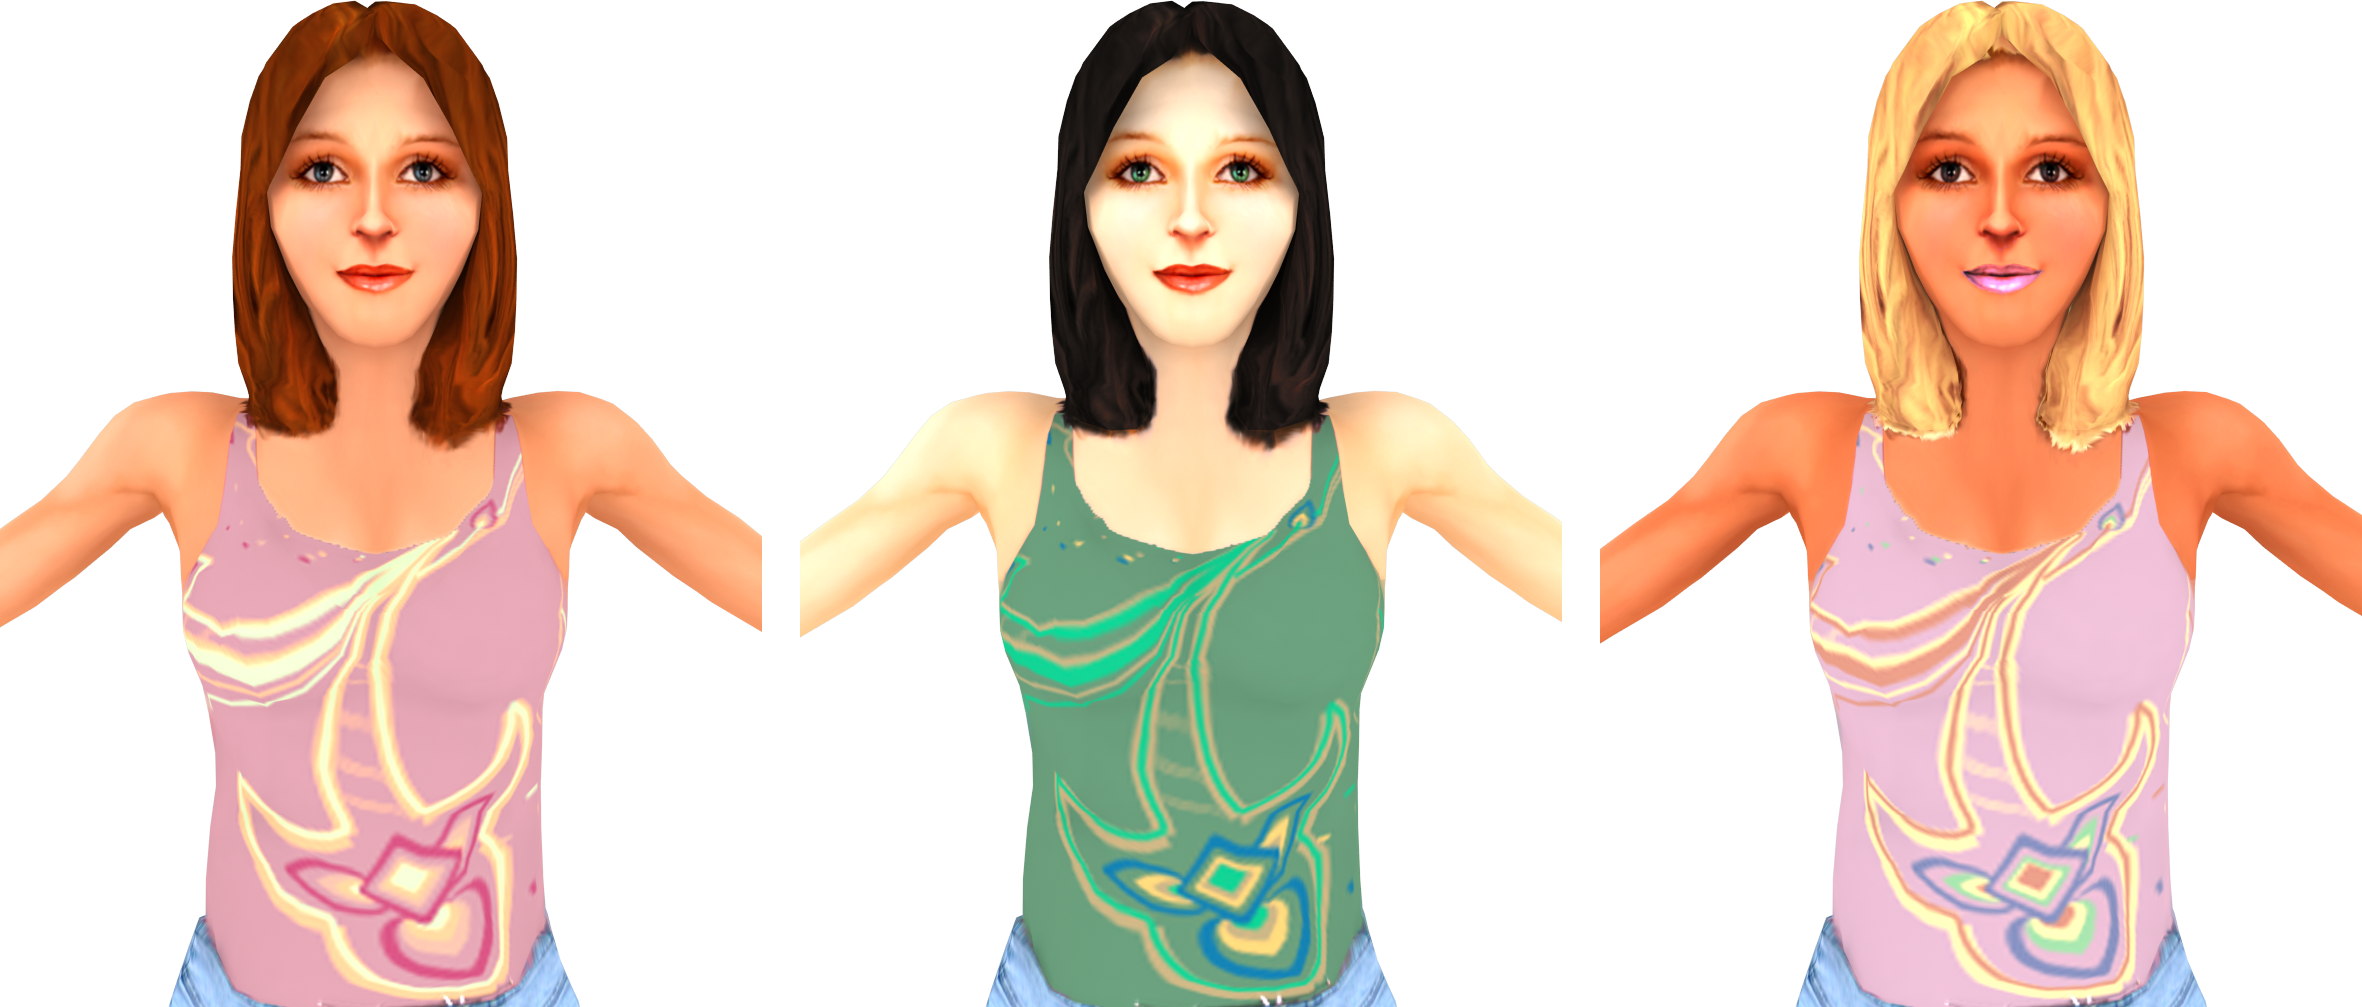
\includegraphics[width=\columnwidth]{figs/fashion/composite}
\caption{Using our model to colorize a patterned shirt for different people. The hair, skin, eye, and lip colors are treated as fixed constraints, which encourage the model to produce compatible colorings via adjacencies and long-range dependencies.}
\label{fig:fashion}
\end{figure}

\subsection{Performance}

The time required to generate coloring suggestions varies depending on the visual complexity of the pattern. With the parallel tempering parameters described at the beginning of this section, it took 73.0s on average to retrieve 20 MMR-diversified results for a single input pattern on a 2.67GHz Intel Core i7. Running time is dominated by MCMC sampling, which on average accounts for 83\% of the total time.

Real-time coloring suggestions would benefit many of the applications demonstrated in this paper, and there are several avenues for improving the performance of our unoptimized, JVM-based prototype to this end. We could leverage the massive parallelism of graphics hardware to speed up parallel tempering, as was done in related work on automatic furniture layout~\cite{MerrellFurnitureLayout}. We could also improve the convergence of the individual MCMC chains via gradient-based proposals, as in Hamiltonian MCMC~\cite{HamiltonianMCMC}.
%Prior work has shown the feasibility of computing the gradients of programmatically-expressed distributions using automatic differentation~\cite{AutoDiff}. 